\documentclass[oneside,14pt]{extarticle}
\usepackage{cmap}
\usepackage[utf8]{inputenc}
\usepackage[english,ukrainian]{babel}
\usepackage{graphicx}
\usepackage{geometry}
\usepackage{listings}
\usepackage{float}
\usepackage{amsmath}
\usepackage{subfig}
\geometry{
	a4paper,
	left=20mm,
	right=20mm,
	top=15mm,
	bottom=15mm,
}
\lstset{
	language=c,
	tabsize=4,
	keepspaces,
	showstringspaces=false,
	frame=single,
	language=C,
}
\graphicspath{ {./pictures} }
\setlength{\parindent}{4em}

\newcommand\subject{Основи програмування вбудованих систем}
\newcommand\lecturer{доцентка кафедри ПЗ\\Марусенкова Т.А.}
\newcommand\teacher{доцент кафедри ПЗ\\Крук О.Г.}
\newcommand\mygroup{ПЗ-32}
\newcommand\lab{2}
\newcommand\theme{Робота з перериваннями на прикладі кнопки на платі STM32F4DISCOVERY}
\newcommand\purpose{Ознайомитися з регістрами для конфігурації переривань, навчитися обробляти зовнішні переривання та читати технічну документацію}

\begin{document}
\begin{normalsize}
	\begin{titlepage}
		\thispagestyle{empty}
		\begin{center}
			\textbf{МІНІСТЕРСТВО ОСВІТИ І НАУКИ УКРАЇНИ\\
				НАЦІОНАЛЬНИЙ УНІВЕРСИТЕТ "ЛЬВІВСЬКА ПОЛІТЕХНІКА"}
		\end{center}
		\begin{flushright}
			\textbf{ІКНІ}\\
			Кафедра \textbf{ПЗ}
		\end{flushright}
		\vspace{80pt}
		\begin{center}
			\textbf{ЗВІТ}\\
			\vspace{10pt}
			до лабораторної роботи № \lab\\
			\textbf{на тему}: <<\textit{\theme}>>\\
			\textbf{з дисципліни}: <<\subject>>
		\end{center}
		\vspace{80pt}
		\begin{flushright}
			
			\textbf{Лекторка}:\\
			\lecturer\\
			\vspace{28pt}
			\textbf{Виконав}:\\
			
			студент групи \mygroup\\
			Коваленко Д.М.\\
			\vspace{28pt}
			\textbf{Прийняв}:\\
			
			\teacher\\
			
			\vspace{28pt}
			«\rule{1cm}{0.15mm}» \rule{1.5cm}{0.15mm} 2024 р.\\
			$\sum$ = \rule{1cm}{0.15mm}……………\\
			
		\end{flushright}
		\vspace{\fill}
		\begin{center}
			\textbf{Львів — 2024}
		\end{center}
	\end{titlepage}
		
	\begin{description}
		\item[Тема.] \theme.
		\item[Мета.] \purpose.
	\end{description}

	\section*{Індивідуальне завдання}
	6. При натисненні користувацької кнопки засвітити червоний світлодіод, при відпусканні — синій.

	\section*{Теоретичні відомості}
	6. Як задати в регістрі SYSCFG\_EXTICR1, щоб оброблялося переривання з виводу 2 порту С?
	
	Щоб налаштувати EXTI2 на використання з портом C, потрібно записати 0010 в біти, що відповідають EXTI2 в SYSCFG\_EXTICR1. Біти для EXTI2 знаходяться на позиціях 8-11 в EXTICR1.
	
	\begin{lstlisting}
	SYSCFG->EXTICR[0] &= ~(0xF << 8);
	SYSCFG->EXTICR[0] |= (0x2 << 8);	\end{lstlisting}
	
	\section*{Хід роботи}
	\subsection*{Створення проекту}
	\begin{figure}[H]
		\centering
		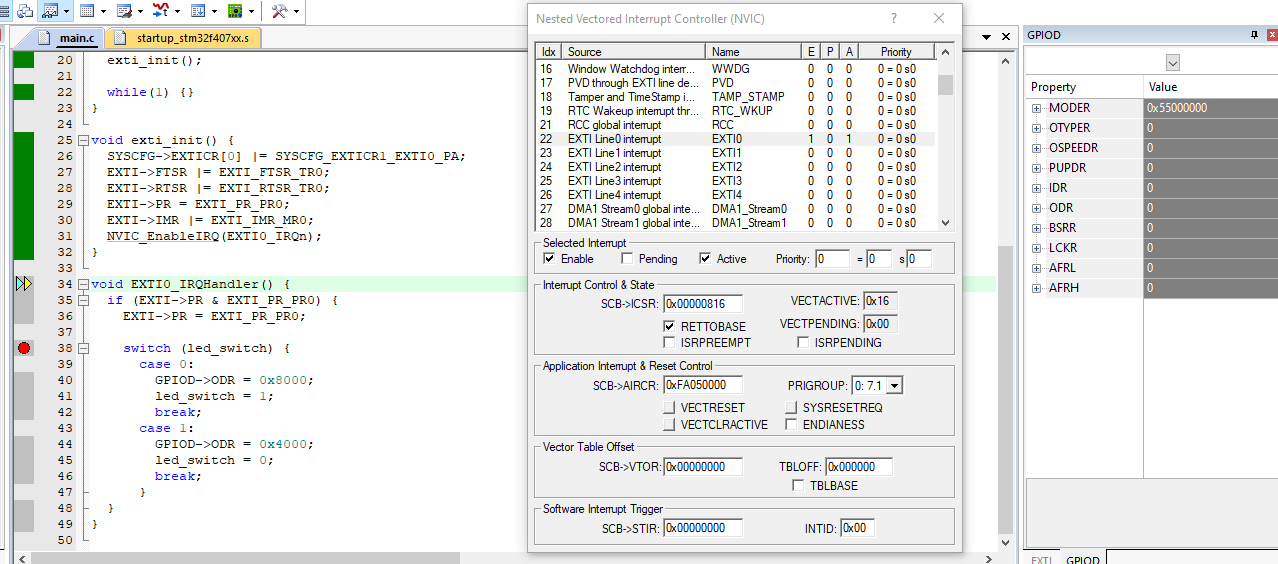
\includegraphics[scale=0.45]{1}
		\caption{Вигляд регістрів ODR до виконання переривань.}
	\end{figure}
	
	\begin{figure}[H]
		\centering
		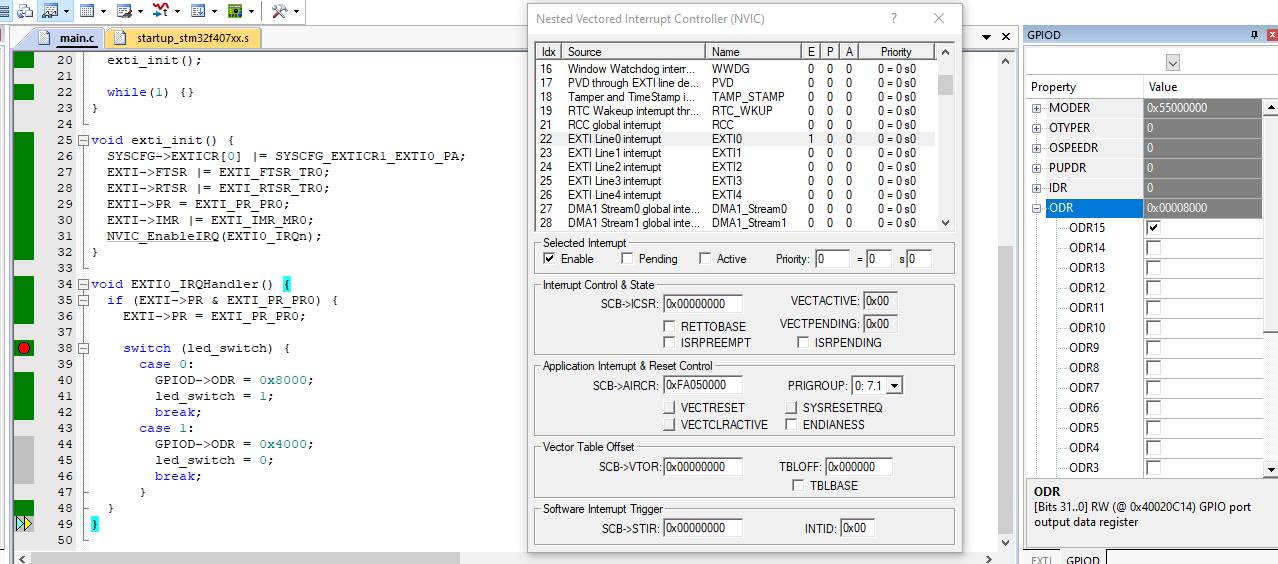
\includegraphics[scale=0.45]{2}
		\caption{Вигляд регістрів ODR після виконяння першого переривання.}
	\end{figure}
	
	\begin{figure}[H]
		\centering
		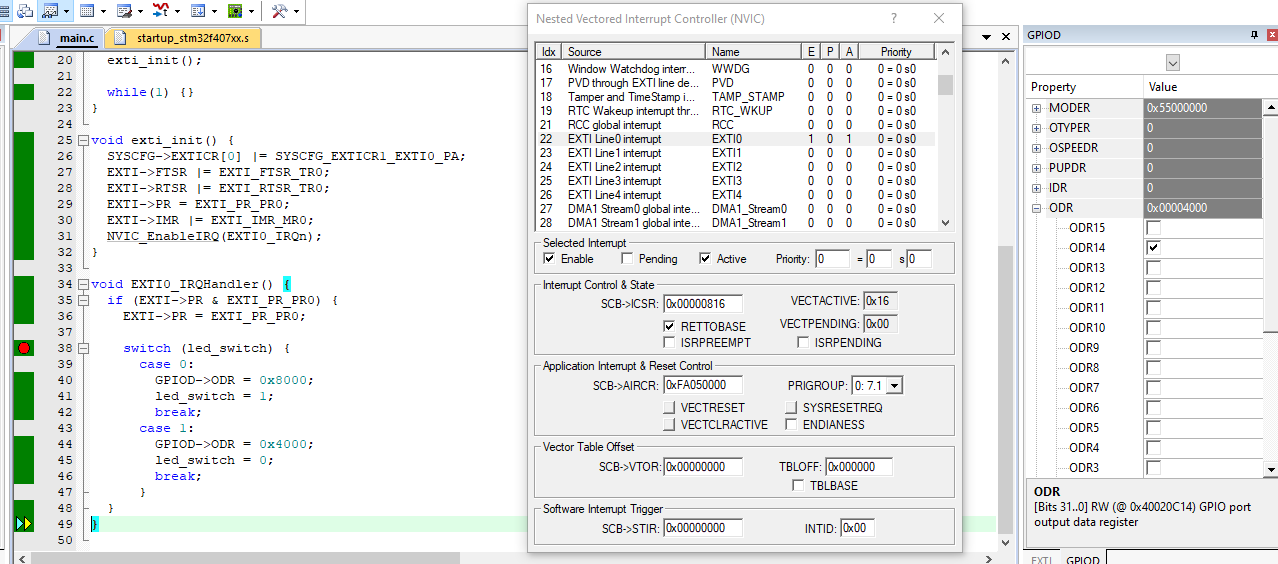
\includegraphics[scale=0.45]{3}
		\caption{Вигляд регістрів ODR після виконяння другого переривання.}
	\end{figure}

	\subsection*{Код програми}
	Файл \textit{main.c}:
	{\small
		\begin{lstlisting}
#include "stm32f4xx.h"
#include <misc.h>

void exti_init(void);
void EXTI0_IRQHandler(void);

static uint32_t led_switch = 0;

int main (void){
	RCC->AHB1ENR |= RCC_AHB1ENR_GPIOAEN;
	RCC->AHB1ENR |= RCC_AHB1ENR_GPIODEN;
	RCC->APB2ENR |= RCC_APB2ENR_SYSCFGEN;
	
	GPIOA->MODER = 0x0;
	
	GPIOD->MODER	= 0x55000000;
	GPIOD->OTYPER = 0;
	GPIOD->OSPEEDR = 0;
	
	exti_init();
	
	while(1) {}
}

void exti_init() {
	SYSCFG->EXTICR[0] |= SYSCFG_EXTICR1_EXTI0_PA;
	EXTI->FTSR |= EXTI_FTSR_TR0;
	EXTI->RTSR |= EXTI_RTSR_TR0;
	EXTI->PR = EXTI_PR_PR0;
	EXTI->IMR |= EXTI_IMR_MR0;
	NVIC_EnableIRQ(EXTI0_IRQn);
}

void EXTI0_IRQHandler() {
	if (EXTI->PR & EXTI_PR_PR0) {
		EXTI->PR = EXTI_PR_PR0;
		
		switch (led_switch) {
			case 0:
			GPIOD->ODR = 0x8000;
			led_switch = 1;
			break;
			case 1:
			GPIOD->ODR = 0x4000;
			led_switch = 0;
			break;
		}
	}
}
		\end{lstlisting}
	}
	
	\section*{Висновки}
	Під час виконання лабораторної роботи я ознайомився з регістрами для конфігурації переривань, навчився обробляти зовнішні переривання та читав технічну документацію.
	    
\end{normalsize}
\end{document}
